\documentclass[varwidth=true, border=2pt]{standalone}
\usepackage{tikz}
\usetikzlibrary{ decorations.markings}

\begin{document}

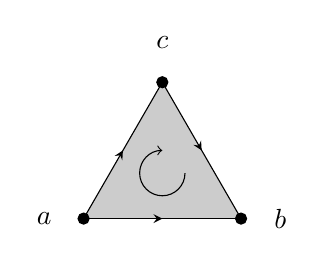
\begin{tikzpicture}
[decoration={markings, 
        mark= at position 0.5 with {\arrow{stealth}[scale=4]}
    }
] 

\coordinate (0) at (0,0);
\coordinate (2) at (2,0);
\coordinate (1) at (1,1.732);
\fill[black!20!white] (0) -- (1) -- (2) -- cycle;
\draw[<-] (1,0.866) arc (90:360:0.288);% syntax (starting point coordinates) arc (starting angle:ending angle:radius)
%\draw  -- (B1) -- cycle;
%\draw (A4) -- (A1) -- (B1) -- cycle;
\draw [postaction={decorate}] (0) -- (1);
\draw [postaction={decorate}] (1) -- (2);
\draw [postaction={decorate}] (0) -- (2); 
%\draw [opacity=0.5,fill=gray] (H) -- (F) -- (C) -- (B)--cycle;
%\draw [opacity=0.5,fill=gray] (E) -- (F) -- (C) --(D)-- cycle;

\node at (-0.5,0) {$a$};
\node at (2.5,0) {$b$};
\node at (1,2.232) {$c$};
\draw[fill=black] (0) circle (2pt);
\draw[fill=black] (1) circle (2pt);
\draw[fill=black] (2) circle (2pt);

\end{tikzpicture}

\end{document}